\chapter{Designing Exergames for Seniors}
\label{chap:exforseniors}

Exergames for elderly has become a popular topic in the past couple of years, and several research on how games can be developed for this particular user group have been conducted. Most of the research done on \ac{hci} are performed on young people \cite{dickinson2007methods}, and it is quite common to develop technology systems for a homogeneous user group. This means that the characteristics of specific user groups, like the elderly, are being ignored. With the wave of elderly ahead of us system designers have to put a greater focus on older people and their needs. Elderly in particular, have some special characteristics due to ageing that needs to be taken into account when developing technology systems for them. Most existing video games have not considered these characteristics, and are therefore not suitable for this group. 

In this chapter we will discuss elderly as a user group of a technology system. We will discuss the characteristics of elderly that are important to acknowledge when designing technology systems for them. Based on previous research done on elderly and exergames, we will draw out some specific guidelines that need to be considered when developing for this group. We will also provide previous research on elderly and user interfaces, as this is an important part of the gaming experience.  In addition, we will present some official guidelines for developing user-friendly interfaces for the elderly user. 

\section{Related Research}
\label{sec:relatedresearch}
There have been done a lot of research on how to make exergames for seniors. In this section we will review some chosen research with interesting findings.

Billis et al. \cite{Billis} discuss some important issues that need to be taken into account when developing games for elderly. Elderly often suffer from decline in visual acuity, decreased audition, mobility changes and cognitive functions' decline. In addition, many elderly are not familiar with technology. The writers suggest that it should be possible to customize the game for every players' special needs. Font, size and color should be adjustable, and information should be provided in different multimedia alternatives, like text, voice and images. The objects should be of sufficient size and the elements should not move too fast. The overall interface should be as simple as possible, without the need to remember information given earlier in the gaming process, and it should be given sufficient information and guidance throughout the whole game. Games should also provide motivating messages to encourage the player. The writers also stress the importance of the social factors of the game, and suggest the ability to multiplay. At last, for the players to get interested and engaged in the game, they suggest that the content of the game should match the users' cultural and lifestyle diversity \cite{Billis}.

de Bruin et al. \cite{bruin} write about the potential of \ac{vr} environment, like exergames, for exercise. \ac{vr} platforms can provide naturalistic movements in a safe environment that can be customized after the patients' needs. It can offer a consistent program that enables for comparison over time. In addition, the use of games can distract the player from any pain they may have. They suggest stepping exercises to be suitable, because they have found that stepping exercises can be a good predictor of falls. It is also proved that a repetitive training program with stepping exercises can improve balance in elderly. Like in other research (sett opp noen kilder jeg finner her), they also here express that the problem of already existing exergames is that they are too complex for the older user group. Therefore, there is a need to develop games specifically for this group where physical and cognitive limitations, as well as typical interests of elderly, are taken into consideration. The writers also present a study where it was shown that there was a significant decrease in relative \ac{dtc} of walking for elderly who was training physically combined with a virtual reality dance game that required decision making, while training traditionally did not change this walking parameters. This comes from the fact that elderly often faces problems when they have to do more than one task at the same time \cite{bruin}.

Brox et al. \cite{exergamesforelderly} suggest some persuasive strategies for motivating elderly to exercise with games. They suggest that too much detailed information about the players progress should be avoided. The information should rather be shown visually, like for example a fish that gets larger and healthier as the player is exercising. Information from previous sessions should be provided, to help players set new goals for the next session. The player should be provided with positive feedback as they achieve goals, and should not be punished if they do not achieve goals. This information and feedback should be given at an appropriate time, and should not  disturb the player. The game should have an easy, understandable and nice interface. The writers see social interaction as very important and suggest that this should be combined with exergaming. This is because it is shown that people get more engaged in the activities when doing it with others and because this group of people often suffer from loneliness and depression \cite{exergamesforelderly}. 

Gregor et al. \cite{gregor} discuss some particular issues when designing for the older population, and propose a paradigm and methodology to support the process of designing software as close to the universal accessibility ideal as possible, which they call \ac{d3} \cite{gregor}.

\cite{gregor} describes older people through three different groups: Fit older people, frail older people and disabled people who grow older. In addition, \cite{gregor} defines some important characteristics of older people:
\begin{itemize}
\item As people get older the individual variability of physical, sensory and cognitive functionality will increase. 
\item Functional decline will go faster when people gets older. 
\item Cognition problems, like memory dysfunction and the ability to learn new things, are widely appearing.
\item Based on where they are in life, elderly may have different wants and needs. 
\item How people live, like if they are needing a walking frame or needing warm glows, can change their usability function.
\item Elderly have more life experience than younger people, and can therefore have more knowledge of the world, as well as a more mature ways of solving problems. 
\end{itemize}

Most software design is static with no possibility to adapt to the different needs of the users. \ac{ucd} principles should be followed when designing technology systems. However, these principles have been developed for homogeneous user groups, and not for specific types of users. To make it easier to develop a technology system for the older user group with different characteristics, \cite{gregor} propose a modified version of the \ac{ucd} principles, which they call \ac{usid}. The issues this methodology address are (Directly drawn from \cite{gregor}): 
\begin{itemize}
\item "Much greater variety of user characteristics and functionality". 
\item "Finding and recruiting "representative users"". 
\item "Conflicts of interest between user groups (including "temporarily able-bodied")".
\item "The need to specify exactly the characteristics and functionality of the user group".
\item "Tailored, personalisable and adaptive interfaces".
\item "Provision for accessibility using additional components (hardware and software)".
\end{itemize}

As an example of the advantages of the proposed methodology, the writers present a case study were a  web browser for people that were visually impaired was developed. 200 visually impaired users evaluated the system.  The findings they did and the conclusions they took out from this study were \cite{gregor}: 
\begin{itemize}
\item Elderly seemed to lack confidence in handling IT systems. However, the confidence increased after they had experienced a successful interaction and decreased after experiencing an unsuccessful interaction.
\item Many elderly had difficulties remembering too much information. This indicates that there are important memory related factors that need to be taken into account when designing for elderly. 
\item Following a need for less information, will most likely also mean less functionality. From an other study they found that it was a need for the possibility that more functionality could be added after the user had mastered the initial, simple functionalities.
\item After some kind of assessment is passed, the user should be moved to a higher level. This can be done for example by self-assessment. To reinforce user-confidence the user should be able to reach goals. 
\end{itemize}

Gerling et al. \cite{gerling1} discuss the chances and challenges when developing a game for the elderly users. They suggest four major guidelines that should be followed when designing games for elderly:
\begin{enumerate}
\item The player should have the possibility to interact with the game both when sitting and standing. 
\item Avoid too extensive and sudden movements.
\item It should be possible to adjust the level when it comes to difficulty, game speed and device sensitivity. This changes should be possible to be adjusted by the player. 
\item Interaction mechanisms should be simple, player frustration should be avoided, and the game should provide constructive feedback.
\end{enumerate}

To verify these guidelines, the research group prototyped an exergame called SilverBalance. This game was made for the Wii Balance Board, consisted of two balance tasks and had the possibility to be played both when sitting and standing. The game was tested on 9 seniors with an average age of 84. The following observations were made \cite{gerling1}.
\begin{itemize}
\item All of the participants were able to play the game adequately. 
\item Participants expressed that the fact that the design was so minimalistic, made it possible for them to focus on the purpose of the game. 
\item The possibility to sit while playing the game was necessary because all participants were dependent on devices to assist them when standing and walking.
\item The players started to compare their results and comment on each others results.
\item Impairments and diseases made it difficult for some participants after a longer period of playing, suggesting that alternative interactions should be included in such games.
\end{itemize}

The testing of SilverBalance shows that the four criteria contributes to the development of exergames for elderly, but that further studies on how age-related changes can affect games, should be carried out \cite{gerling1}.

In another study Gerling et al. present a case study where they introduce and evaluate another video game for elderly, called SilverPromenade \cite{gerling2}.  SilverPromenade is developed for the Nintendo Wii technology and utilizes the Wii Remote and Wii Balance Board. The game is stripped from complexity in functionality and design to be senior-friendly. The theme of the game is "a walk through the forest" and it can be played as a single-player game or a multi-player game. In each mode of the game it is possible to engage three different roles, walking through the forest by stepping on the Wii Balance Board which requires physical exercise, catching a butterfly by pointing at it with the Wii Remote, and counting rabbits by shaking the Wii Remote when a rabbit appears. The scenarios are simplistic, which is important when including elderly in digital game play. The concept of the game, "a virtual walk in the forest", was chosen because it appeals to elderly living in nursing-homes because it offers the possibility to "visit" the forest, which generally might be inaccessible for them. Playing this game requires the older player to focus on cognitive, mental and physical abilities. They have to understand the basics of the game, they have to pay attention to elements appearing on the screen, and they have to be prepared for challenging situations. 

SilverPromenade has an easy and understandable user interface. Complex graphics and visual effects are avoided, while important elements are highlighted. It consists of a menu structure which easily guides the user to the playing-mode. The input devices used for playing makes it possible for elderly to both sit and stand during game-play, which takes the different individuals abilities into consideration.  If one of the three roles is not suitable, SilverPromenade offers the possibility of not including one or more roles.

A case study with SilverPromenade was executed on a group of frail elderly living in full-time nursing homes. The participants were asked to play the game and afterwards fill out a short questionnaire. During the case study they examined three research question related to interface design, game design, and player experience. Two groups of elderly participated, one group with prior experience with this type of technology, and one group without any experience. The participants suffered from age-related changes, and most of them needed assistive devices to walk. During the game play the researchers observed how the elderly used the controllers, how they understood the menu, and how easily they perceived the game behaviour. The gaming results were also observed.

Results from this case study show that experienced players clearly had an advantage over the inexperienced players. It was observed during game-play that some roles were difficult to execute. When walking on the Balance Board they experienced difficulties with performing correct movements, and when pointing at the butterflies they had difficulties using the Wii Remote because it requires that one point it directly towards the sensor. However, the results showed that the overall experience was positive. SilverPromenade gave an impression of being outside, and the use of a real-world scenario engaged elderly to play. The concept of the game lead to communication in terms of identifying objects, and helping and encouraging each other. One important observation was that the elderly where sharing and discussing their scores. The conclusion of the case study was that elderly enjoyed playing digital games, and that SilverPromenade could be an appropriate game to use in this age group \cite{gerling2}.

Most studies done on elderly and the use of digital games suggest that social interaction is important to include. Social interaction can be multi-play both in person in the same room and online. Online multi-play could be a good way to socialize for elderly who are less mobile and are lonely. However, not many studies on playing games together over the internet have been conducted. We do now that elderly often are unfamiliar with this type of technology \cite{Billis}, \cite{gregor}, and it is therefore important to acknowledge the challenges that can be faced by introducing multi-play over the internet for this group. Gajadhar et al. \cite{Gajadhar} did a study, where they wanted to find out how players experiences playing together with different social presence. They tested a digital game on 40 participants in pairs with three different degrees of social presence: \emph{co-located co-play}, which means playing in the same room at the same time, \emph{virtual co-play}, which is playing against a computer controlled player, and \emph{mediated co-play}, which is playing together online. Results showed that while playing online elderly experiences low enjoyment, competence and challenge score, which indicates that they did not like playing online. It was also shown that they had more fun when playing alone, than when playing online with others. When playing together with others, they preferred seeing their co-players, and be able to speak with them. Seniors experienced more fun, competence, challenge and immersion when playing together in the same room than when playing with others over the internet. It was also found that seniors seemed to not care if they were winning or losing. They appeared to not be very competitive.  Instead they enjoyed helping each other. The writers links this to previous studies that had found that elderly rather liked to help and teach others how to play games, than compete. The writers suggest that when including social interaction in games, the focus should be on cooperation rather than competition \cite{Gajadhar}. 


\section{Summary of Findings from Related Research}
\label{sec:summaryguidelines}
It is clear from the literature that elderly has some specific characteristics that need to be considered when developing technology systems aimed for them. Based on the reviewed research we will summarize these characteristics and also the different guidelines proposed.

\subsection{Characteristics of elderly people:}
\label{subsec:characteristics}
\begin{enumerate}[{c}.1]
\item Cognitive functions' decline, e.g. dementia, memory dysfunction, and the ability to learn new things \cite{Billis}, \cite{gregor}.
\item Decline in sensory functionality, like  visual acuity and audition \cite{Billis}, \cite{gregor}.
\item The problems elderly face, often increase significantly with increasing age \cite{gregor}.
\item Mobility change \cite{Billis}.
\item Needs and wants related to cultural and lifestyle diversity, as well as at what stage they are in life \cite{Billis}, \cite{gregor}.
\item Many are in need of assistive tools (for example when standing and walking) \cite{gregor}.
\item Inexperienced with technology. Many elderly seems to lack confidence when it comes to IT-systems. A better confidence can be achieved when experiencing a successful interaction with an IT-system \cite{Billis}, \cite{gregor}.
\item It is important to take into account memory related factors. Many elderly have difficulties remembering too much information \cite{Billis}, \cite{gregor}.
\item It can be hard to do two things at the same time \cite{bruin}.
\end{enumerate}

\subsection{Guidelines to follow when designing exergames for elderly}
\label{subsec:guidelines}

\begin{enumerate}[{g}.1]
\renewcommand{\labelitemi}{$\bullet$}
\item The game should have the possibility to be customized for every user's needs, condition, interests etc.. This can be done by offering alternative interactions \cite{Billis}, \cite{gregor}, \cite{gerling1}.
\item Offer adjustable font, size and colors \cite{Billis}.
\item The interface should have different alternatives for multimedia presentation, for example, text, voice and images \cite{Billis}.
\item The interface should be simple and not too extensive. The objects should be of sufficient size and there should be no sudden movements. Important elements should be highlighted \cite{Billis}, \cite{gerling1}, \cite{gerling2}, \cite{exergamesforelderly}.
\item Sufficient guidance and information should be given during the process, without the need to remembering earlier given information \cite{Billis}, \cite{gregor}.
\item Constructive feedback should be given in a motivating form, to encourage play \cite{Billis}, \cite{gerling1}, \cite{exergamesforelderly}.
\item The story of the game should match cultural and lifestyle diversity. An example presented in \cite{gerling2} is a game with a real-world scenario, where the players have to walk through a forest. This seemed to appeal to elderly living in a nursing home, because they do not have the same possibility to "just take a walk" in the forest \cite{Billis}, \cite{gregor}, \cite{gerling2}. 
\item Social factors should be included, by for example offering the possibility to multiplay \cite{Billis}, \cite{gerling2}, \cite{gerling1}, \cite{exergamesforelderly}.
\item Multi-play should focus more on cooperation than competition \cite{Gajadhar}.
\item It should be offered variety in user characteristics and functionality \cite{gregor}, \cite{gerling1}.
\item The game should not have too much functionality, but instead offer the possibility to add more functionality after the existing functionalities are managed \cite{gregor}, \cite{gerling2}.
\item Offer different levels with different difficulties. With this comes the possibility to reach goals. The device sensitivity and the game speed should also be adjustable \cite{gregor}, \cite{gerling1}.
\item It should be possible for the player to adjust levels themselves \cite{gregor}, \cite{gerling1}. 
\item It is important during the development to test on representative users \cite{gregor}.
\item The possibility to interact with the game both when sitting and standing is important \cite{gerling1}, \cite{gerling2}.
\end{enumerate}

As an additional guideline, it is worth mentioning that both in \cite{bruin} and \cite{gerling2} they discuss stepping as a relevant exercise for elderly. This is because this kind of exercise has proved to be a good predictor of fall and that repetitive stepping exercises can improve balance. In addition stepping requires significant physical activity, which is important when improving physical health. Walking or stepping exercises is also recommended by the Department of Health and Human Services, discussed in Chapter \ref{chap:olderexercise}.


\section{Official Guidelines for Designing User-Friendly Interfaces for Elderly Users}
\label{sec:designelderly}

As listed as characteristics in the previous section, ageing will often lead to both physical and psychological negative changes, like decline in cognitive skills, visual and auditory acuity, and in balance and physical strength. Many elderly also experience memory loss, and difficulties moving around due to decreased flexibility. An important part of game development is designing the user interface. When working on interface design, visual decline may be the most important aspect to focus on. Visual decline implies less contrast sensitivity, decrease in peripheral vision, and more dark adoption (KILDE). 

There exist various examples of guidelines for how to design good and user-friendly interfaces for elderly, or people in general, that are partially sighted or visually impaired. Some of the main guidelines are simple design, large font size, and sharp contrast between background color and font color. The users might have different levels of visual decline, so it is preferable to allow users to change settings themselves \cite{blindeforbundetTekst} \cite{actionforblindpeopleTekst} \cite{w3cTekst}. Design guidelines are provided by various organisations, as e.g. "Blindeforbundet", a Norwegian federation for everyone with poor vision \cite{blindeforbundet}, "Action for Blind People", a charity in the UK which provides support to people that are blind or partially sighted \cite{actionforblindpeople}, and "World Wide Web Consortium (W3C)", a community working together to create web standards \cite{w3c}. These web standards are meant to be used as guidelines for making usable interfaces for the general user, regardless of age or disabilities \cite{w3cTekst}. These three organisations are just a few out of several others with focus on making technology accessible for elderly and people with visual disabilities. 

We will now present a summary of guidelines to consider when designing an interface for elderly, mostly gathered from the three organisations mentioned above.

\begin{figure} [ht!]
\centering
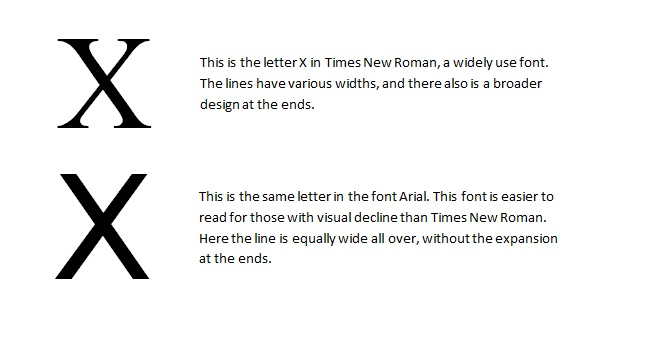
\includegraphics[scale=0.9]{fontExample.jpg}
\caption[Fonts]{Font with and without serifs [modified from \cite{blindeforbundetTekst}]}
\label{fig:fonts}
\end{figure}

\textbf{Make the text easy to read}
\begin{enumerate}[{o}.1]
\item Use a relatively large font size, minimum 12 pt \cite{blindeforbundetTekst} \cite{evengrounds}. A font size of 14-16 pt is preferable for those who are visually impaired. For large prints use 16-22 pt \cite{actionforblindpeopleTekst}. Use of font size larger than 20 pt will not increase readability in a text.     
\item Use a clear print. This mean that a sans serif font should be used, see Figure \ref{fig:fonts}. Arial, Helvetica and Futura are fonts that are easy to read \cite{actionforblindpeopleTekst}.
\item Avoid fonts with special styles \cite{blindeforbundetTekst} \cite{actionforblindpeopleTekst}.
\item For titles, use upper-case letters in beginning of words \cite{actionforblindpeopleTekst}. Do not use capital letters in large amounts. They give little variation, which makes the text difficult to read \cite{blindeforbundetTekst}. 
\item Do not use italics, underlining and bold typing in a larger coherent text, that will disturb the reading \cite{blindeforbundetTekst} \cite{actionforblindpeopleTekst}.  
\item If possible, allow the users to change font and text settings themselves \cite{blindeforbundetTekst} \cite{w3cTekst}. 
\item Use a language with ordinary, well-known words. This makes the text more easy to understand \cite{w3cTekst}. \\ 


\textbf{Use simple design}

\item Use simple design, as this makes it easy for important elements to stand out \cite{actionforblindpeopleTekst}.
\item Be consistent in design and layout throughout the system \cite{actionforblindpeopleTekst}.
\item Always use left-aligned text. Centered text appears unclear \cite{actionforblindpeopleTekst}.  
\item Keep spacing between words permanent. Do not stretch the text to get an even right margin, as this will change the spacing randomly. An uneven right margin is good for readability, as it help leading the eyes to the next line \cite{blindeforbundetTekst} \cite{actionforblindpeopleTekst}.
\item Do not use to much or to little spacing between lines \cite{blindeforbundetTekst} \cite{actionforblindpeopleTekst}. 
\item Avoid big blocks of text. The text will be easier to read and understand if it is divided into smaller sections \cite{blindeforbundetTekst} \cite{actionforblindpeopleTekst} \cite{evengrounds}. \\  


\textbf{Use of colors and contrasts}
\item It is important with sharp and clear contrast between background color and font color to ensure good readability \cite{blindeforbundetTekst} \cite{actionforblindpeopleTekst}. The actual choice of colors is not that essential.   
\item In general, the most preferred combination of background color and font color is black text on either white or yellow background \cite{actionforblindpeopleTekst}. Black on white or yellow creates very good contrast \cite{blindeforbundetTekst}. 
\item People are different. Some might prefer the opposite, like light font colors on dark background \cite{blindeforbundetTekst}. This again emphasises that it should be possible to customise settings. When using light font colors on dark background, the font should be both bigger and bolder to make the text more readable \cite{actionforblindpeopleTekst}.
\item Avoid pale colors on colored background \cite{blindeforbundetTekst}.  
\item Choose a one-colored background. Try not to write text on pictures. The picture will take the attention away from the text, and make the text harder to read. If necessary, put the text where there is light areas in the picture  \cite{blindeforbundetTekst}.  
\item Reading speed and distant reading is also highly connected to colors and contrast  \cite{blindeforbundetTekst}. Black text on white background provides the highest reading speed in a text. For more combinations, see Figure \ref{fig:colors}.


\begin{figure} [ht!]
\centering
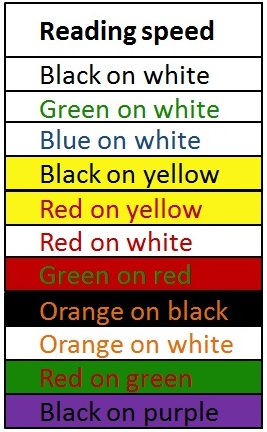
\includegraphics[scale=0.5]{readingcolors.jpg}
\caption[Colors and contrasts]{Relationship between reading speed and distant reading, and colors and contrasts. The best combinations are those shown on top [translated from Norwegian, \cite{blindeforbundetTekst}]}
\label{fig:colors}
\end{figure}

\textbf{Provide necessary information}
\item Provide alternatives for how to present information. For those who are visually impaired, an audio presentation might be preferable \cite{blindeforbundetTekst} \cite{w3cTekst}. 
\item Text is a better way to present information than use of images and icons \cite{w3cTekst}.
\item Give the users time to read the given information. Let them tell the system when they are finished reading \cite{w3cTekst}.  
\item Help users to easily navigate to the the content of interest \cite{w3cTekst}.
\item Assist users on how to avoid and correct mistakes. Describe the error for the user, and provide a suggestion for how they can undo the action that caused the error \cite{w3cTekst}.      
\end{enumerate} 

The characteristics and guidelines drawn from previous studies together with the official guidelines proposed by "Blindeforbundet", "Action for Blind People" and "World Wide Web Consortium (W3C) will become very important  when we develop a concept for an exergame for elderly. To understand how to design this exergame, we also have to understand how video games in general can be designed. This will be described in the next chapter.




